\addchap{Grußwort}

\begin{wrapfigure}{l}{0.32\textwidth}
  \vspace{-15pt}
  \begin{centering}
    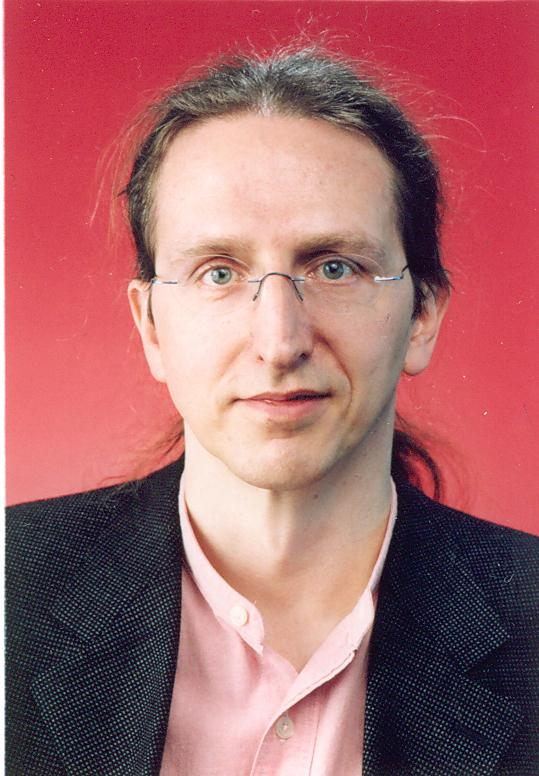
\includegraphics[width=0.3\textwidth]{img/franzbaader.jpg}
  \end{centering}
  \vspace{-20pt}
\end{wrapfigure}

Liebe Studentinnen und Studenten,

als Dekan der Fakultät Informatik ist es mir eine Freude, Sie herzlich zur Aufnahme Ihres Studiums an unserer Fakultät zu begrüßen. Mit 28 Professoren, 4 Honorarprofessoren, mehr als 300 Mitarbeitern und mehr als 1600 Studenten gehört die Fakultät zu den größten Informatikfakultäten Deutschlands. Um unser modernes Gebäude werden wir von vielen anderen Fakultäten beneidet, auch wenn es manchmal als Grünes Gewölbe bezeichnet wird. Ich kann Ihnen aus eigener Erfahrung versichern: man gewöhnt sich an die Farbe. Das Gebäude bietet nicht nur Platz für die Mitarbeiter der Fakultät, sondern verfügt auch über einen Vorlesungssaal, diverse Seminarräume und hochwertig ausgestattete Rechner-Pools. Im Foyer liefert das Studentencafe ASCII den für einen Wissenschaftsbetrieb äußerst wichtigen Koffeinnachschub.

Die Informatik durchdringt unsere Gesellschaft wie keine andere Wissenschaft und beschleunigt den wissenschaftlichen Fortschritt anderer Disziplinen enorm. Software läuft nicht nur in dedizierten Computern, sondern auch in Autos, Flugzeugen, Wasch- und Kaffeemaschinen. Computerprogramme erledigen heute Aufgaben, die noch vor 20 Jahren Biologiestudenten einen Doktortitel eingebracht hätten. Teilweise ist die Durchdringung sogar so tief, dass sie der Gesellschaft gar nicht mehr bewusst ist. Die kürzlich gehörte Frage eines Kindes „Papa, wie kam man eigentlich ins Internet, bevor es Computer gab“ ist hierfür nur ein Beispiel. Sie führt aber dazu, dass in vielen Bereichen Firmen händeringend nach Informatikern suchen. Unsere Fakultät kann derzeit mit unseren Absolventen nicht einmal den Fachkräftebedarf der Industrie im Raum Dresden decken. Nach dem erfolgreichen Abschluss Ihres Studiums werden Ihnen daher viele Türen offenstehen. Ich hoffe jedoch, dass Sie sich nicht nur wegen der guten Job-Aussichten für das Studium der Informatik entschieden haben, sondern auch wegen Ihres Interesses am Fach und der Freude am Lernen. Wir freuen uns auf jeden Fall darauf, Sie zu lehren.

Für Sie, liebe Studentinnen und Studenten, beginnt mit dem Studium ein neuer Lebensabschnitt, der mehr Freiheiten bietet als die Schule vorher und das Berufsleben nachher. Nutzen Sie diese, aber missbrauchen Sie diese nicht. Sie haben mehr Freiheit, sich die Arbeit einzuteilen, doch aus eigener Erfahrung kann ich Ihnen versichern, dass ein erfolgreiches Studium mehr Aufwand erfordern wird, als Sie das von der Schule gewohnt sind. Gehen Sie regelmäßig in die Vorlesungen, bereiten Sie diese nach und erarbeiten Sie sich die Lösungen zu den Übungsaufgaben selbstständig. Das erfolgreiche Herunterladen der Vorlesungsfolien oder des Skripts zur Vorlesungen trägt wenig zum Bestehen der Prüfung bei, wenn Sie sich nicht intensiv mit den Inhalten auseinander setzen. Versuchen Sie nicht, das Studium als Einzelkämpfer zu bewältigen. Nutzen Sie die Tatsache, dass Sie an einer großen Fakultät zusammen mit vielen Kommilitonen studieren, um mit diesen Vorlesungsinhalte zu diskutieren und sich schwierige Themen gemeinsam zu erarbeiten. Das verbessert nicht nur den Studienerfolg, sondern macht auch viel mehr Spaß. Wenn Sie trotzdem im Studium auf Probleme stoßen, stehen Ihnen viele Anlaufstellen zur Verfügung: Studienberater, Mitglieder des Fachschaftsrates, Übungsgruppenleiter und selbstverständlich auch alle Professoren. 

Das Humboldtsche Bildungsideal der Einheit von Forschung und Lehre spielt auch an der Fakultät Informatik der TU Dresden eine wichtige Rolle. Die Professoren und wissenschaftlichen Mitarbeiter der Fakultät arbeiten nicht nur in der Lehre, sondern beschäftigen sich im Rahmen einer Vielzahl von Drittmittelprojekten intensiv mit Forschungsthemen in verschiedensten Grundlagen- und Anwendungsbereichen. Seit dem 15. Juni 2012 ist die TU Dresden wegen ihrer herausragenden Forschungsleistung in den Kreis der Exzellenzuniversitäten aufgestiegen.  Die Fakultät Informatik ist im Exzellenzcluster „Center for Advancing Electronics Dresden“  zentral beteiligt. Ziel ist dabei die Entwicklung neuer Technologien für die elektronische Informationsverarbeitung der Zukunft,  welche die Begrenzungen heutiger CMOS-Technologie überwinden. Dabei forschen die Informatiker an Techniken, die sichere Berechnungen auch mit fehleranfälliger Hardware ermöglichen, sowie an Techniken zur Handhabung von Systemen mit sehr vielen und heterogenen Chips.  Im Rahmen des Exzellenzclusters wurden an der Fakultät Informatik zwei neue Professuren für Prozessordesign und Compilerbau geschaffen, die auch die Studienbedingungen an der Fakultät, z.B. mit einem erweiterten Vorlesungsangebot, noch weiter verbessern. Die Fakultät war zusätzlich erfolgreich in der Einwerbung zweier Doktorandenprogrammen, sogenannter Graduiertenkollegs, in den Bereichen Theoretische Informatik und Software Engineering bei der Deutschen Forschungsgemeinschaft. Sie ist damit die einzige Informatikfakultät Deutschlands, die zwei solche prestigeträchtige Programme gleichzeitig anzubieten hat. Aber auch andere Drittmittelprojekte sowie vom Land finanzierte Stellen bieten Ihnen Finanzierungsmöglichkeiten dafür, im Anschluss an Ihr Studium an der TU Dresden zu promovieren.

Die erwähnten vielfältigen Forschungsaktivitäten der Fakultät stehen nicht in Konkurrenz zur Lehre, sondern ergänzen diese in vielerlei Hinsicht, auch wenn Sie davon nicht unbedingt bereits in den ersten Semestern profitieren. Die Forschungsprojekte ermöglichen es Ihnen, im Rahmen von Projekt- und Abschlussarbeiten oder als (bezahlte) studentische Hilfskraft an der Lösung aktueller Forschungsfragen mitzuarbeiten. Die durch die Projektarbeit entstandenen Kontakte zur Projektpartnern in der Industrie oder an anderen akademischen Einrichtungen bieten Ihnen die Möglichkeit zu Industriepraktika und Auslandsaufenthalten. Und Sie erfahren in fortgeschrittenen Vorlesungen teilweise die neuesten Ergebnisse aus erster Hand, von den Leuten die sie erzielt haben.

Am Ende meines Grußwortes möchte ich mich ganz herzlich beim Fachschaftsrat für das große Engagement in der Fakultät und insbesondere für die Durchführung der Erstsemestereinführung bedanken. Die Fakultät lebt vom Engagement aller Mitglieder, insbesondere ihrer Studenten. Sie bekommen von uns ein vielfältiges Angebot. Bitte nutzen Sie es so gut wie möglich und gestalten Sie mit uns die Zukunft der Informatik!

\textit{Franz Baader,\\
Dekan der Fakultät Informatik}

\vfill

\begin{figure}[h!]
\centering
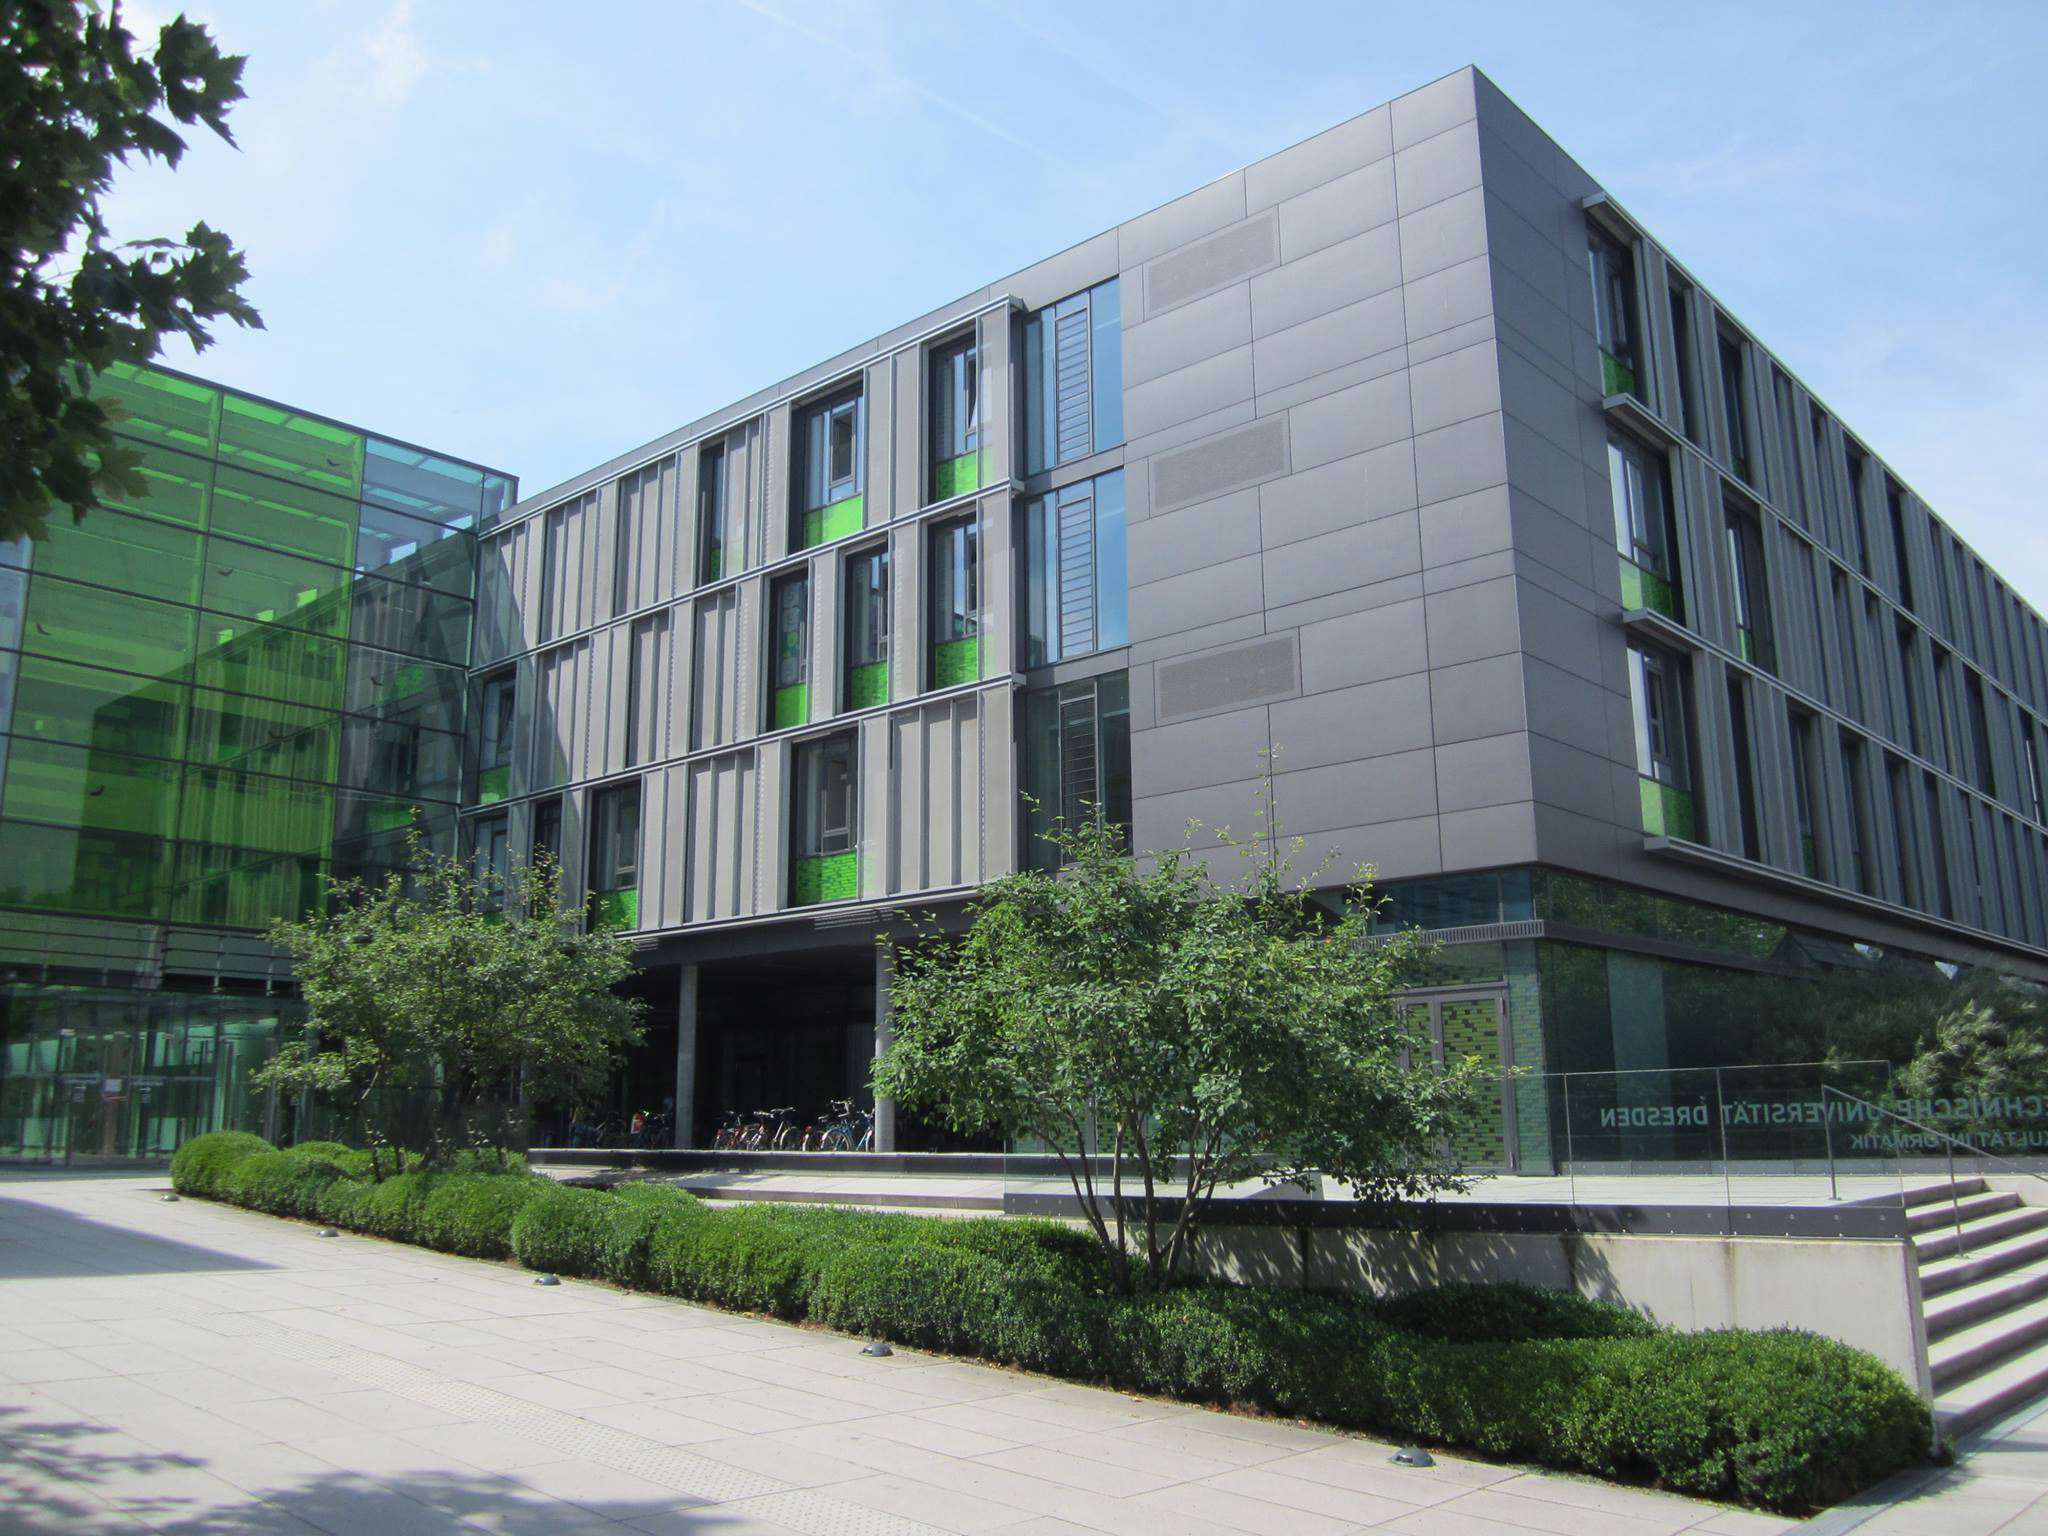
\includegraphics[width=.9\linewidth]{img/fakultaet.jpg}
\caption*{{\small Fakultät Informatik - Foto: Philipp Heisig}}
\end{figure}
